\section[Data Monitoring]{Aim 3 - Health System Data Monitoring and Screening}

The third aim of my dissertation is the development of methods for screening and monitoring of data collected in health systems to inform and orient supervisions. Specifically, I will consider data collected in \gls{rbf} programs in Bénin. \gls{rbf} is a mode of financing of health systems based on the ex-post payment of health facilities by a national financing body or program. This mode of financing alleviates the burden of planning for coordinating bodies, but transfers it to increased reporting needs for facilities. In order to receive these payments, facilities have to report monthly on a set of indicators on which these payments will be based \citep{musgrove_financial_2011}.

In a \gls{rbf} system, understanding and monitoring results is thus important on two main levels. First, Program managers want to have an accurate evaluation of the activity they should be paying for, as the accurate evaluation of this amount is key to the success of the program. Underfinancing facilities endangers their ability to operate in good conditions, but overpaying some facilities may be detrimental to the overall sustainability of the project. Second, being able to measure and compare facilities performance is essential to identify weakly performing facilities, and to start implementing correcting measures.

In Bénin, the \gls{prss} has been launched in 2011 by a consortium formed by the Beninese government, the World Bank, the GAVI Alliance and the Global Fund. As part of this program, a comprehensive \gls{rbf} program has been implemented in all 34 health zones of the country. To allow the management of RBF reporting data, the software OpenRBF, developed by the Belgian startup Bluesquare has been implemented.

In systems using OpenRBF, data is collected in facilities for indicators contracted in the \gls{rbf} program, and are reported at district level on a monthly basis. The District administrators are in charge of entering the data in the OpenRBF database. This monthly data is then aggregated, and checked on a quarterly basis for quality. Data quality check is made through a field visit made by project managers in facilities, who will then check the quality of primary data collection in facilities (reports, charts) and the quality of reporting, by comparing collected primary data and reported numbers.

This system allows to improve the confidence and exactitude of reported numbers, on which payments to facilities depend. Meanwhile, it is costly and does require regular field visits by program managers \citep{antony_exploring_2017}. This system has proved its worth in allowing \gls{rbf} program managers to access credible data on facilities performance. Meanwhile, in a program managing close to 800 facilities, it is increasingly unceasingly difficult to validate data, and to monitor service quality. I will develop an approach to screen indicators reported by facilities, to help program managers making decisions. The decision framework in which we operate is quite simple, and has two main outcomes : validate data or not, raise a service quality issue or not. These two outcomes are not independent, and all depend on an evaluation of the normality of reported data when compared to previously observed data.

\subsection{Research questions}

This project will be aimed at developing and validating a generic framework for screening and validating data reported by facilities in the Bénin RBF program. I will develop this framework in three specific objectives.

\begin{description}
	\item[Data screening] In a first step, I will implement and compare different approaches to data monitoring in order to detect and report anomalies in the observed series. Combining methods used for syndromic surveillance, health system performance monitoring, and industrial \gls{spc}, I will define an algorithm to screen reported data, and spot abnormal values.
	\item[Classification] In a second step, I will test a classification method to differentiate spotted abnormalities between data quality issues and other issues.
	\item[Program Management] Finally, I will simulate different strategies to prospectively collect data in facilities, so as to allow an optimal performance of imputation models at a minimum cost.
\end{description}

\subsection{Data}
\label{paper2_data}

OpenRBF has been implemented in Bénin since March 2012, and has been rolled out in every départements of the country. Data is collected and validated monthly for the \gls{pma}, which is a minimum package of services that includes most standard primary care activities (immunization, antenatal care, malaria care). As of January 2017, the data consists in 16131 facility/months of \gls{pma} data in 671 different facilities. In each report, a median of 75\% of indicators are correctly reported, as shown in figure \ref{fig:dist_percent_correct}.

\begin{center}
\begin{figure}[ht]
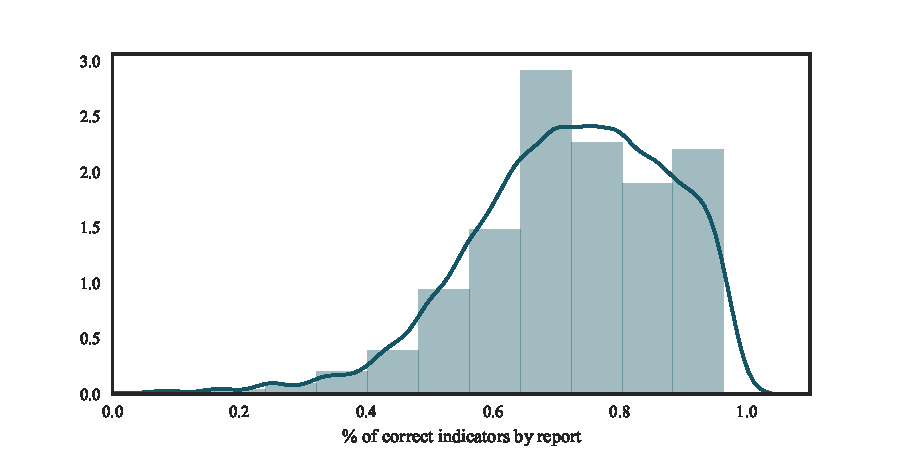
\includegraphics[width=\textwidth]{figure/correct_dist.pdf}
\caption{Distribution of the percentage of correct indicators by report}
\label{fig:dist_percent_correct}
\end{figure}
\end{center}

Figure \ref{fig:facility_correction_distribution} shows the distribution of the amounts by which payments have been corrected after data validation. We see that the distributions are skewed on the left, showing that most corrections lead to diminutions of the amounts. In the meantime, the distributions are very peaked around a mean close to 0, which leads me to hypothesize that most of the corrections can be attributed to situations of reported  service provision that could not be fully documented, and a can thus be understood as data quality issues more than deliberate data manipulation.

Figure \ref{fig:facility_correction_evolution} shows the evolution of monthly correction amounts percentage for the same facilities. The pattern of these evolutions is similar for each facility, and suggests an \textit{in control} state with low variance, and some episodes of aberrant values. Some of these \textit{out of control} situations appear to have some persistance as the early 2014 in the CSA Kpasse. My work will be to detect these episodes based on reported data.

\begin{center}
\begin{figure}[ht]
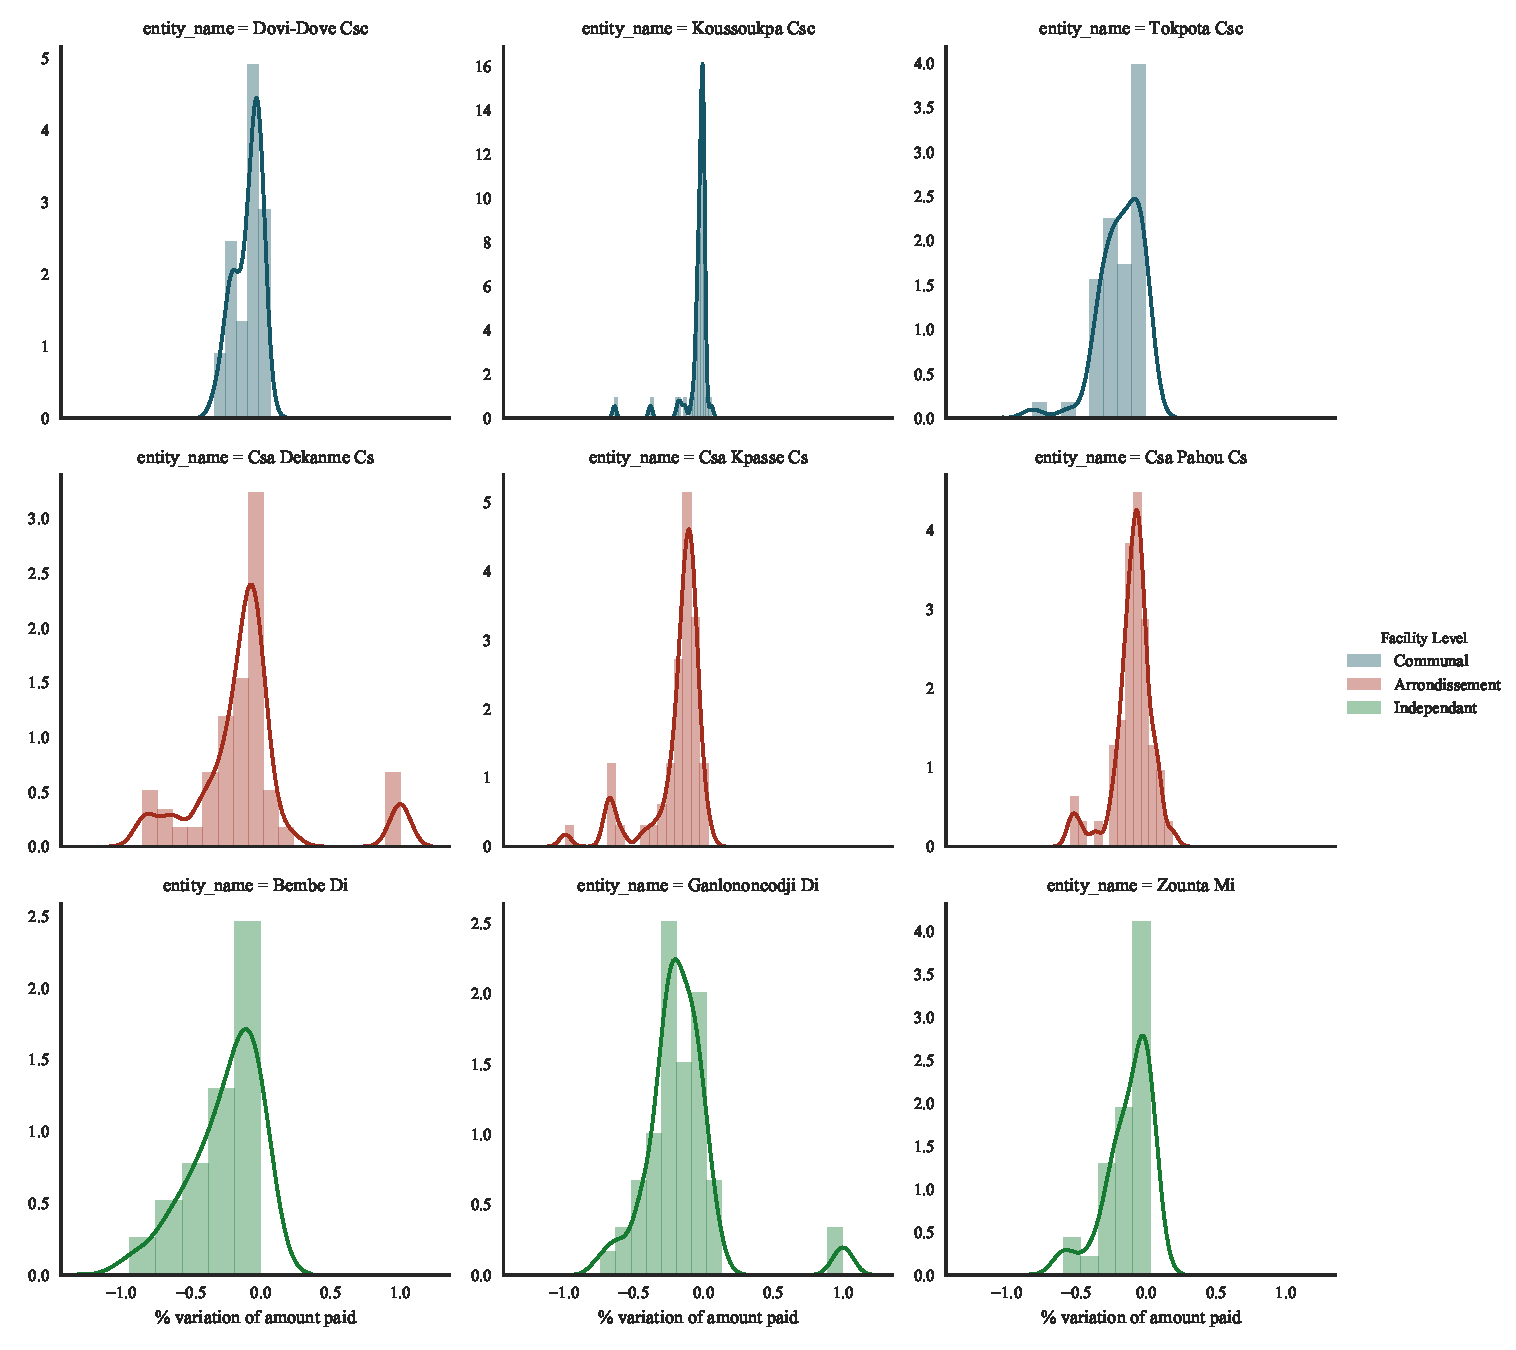
\includegraphics[width=\textwidth]{figure/facility_correction_distribution.pdf}
\caption{Distribution of payment correction percentage for a sample of indicators}
\label{fig:facility_correction_distribution}
\end{figure}
\end{center}

\begin{center}
\begin{figure}[ht]
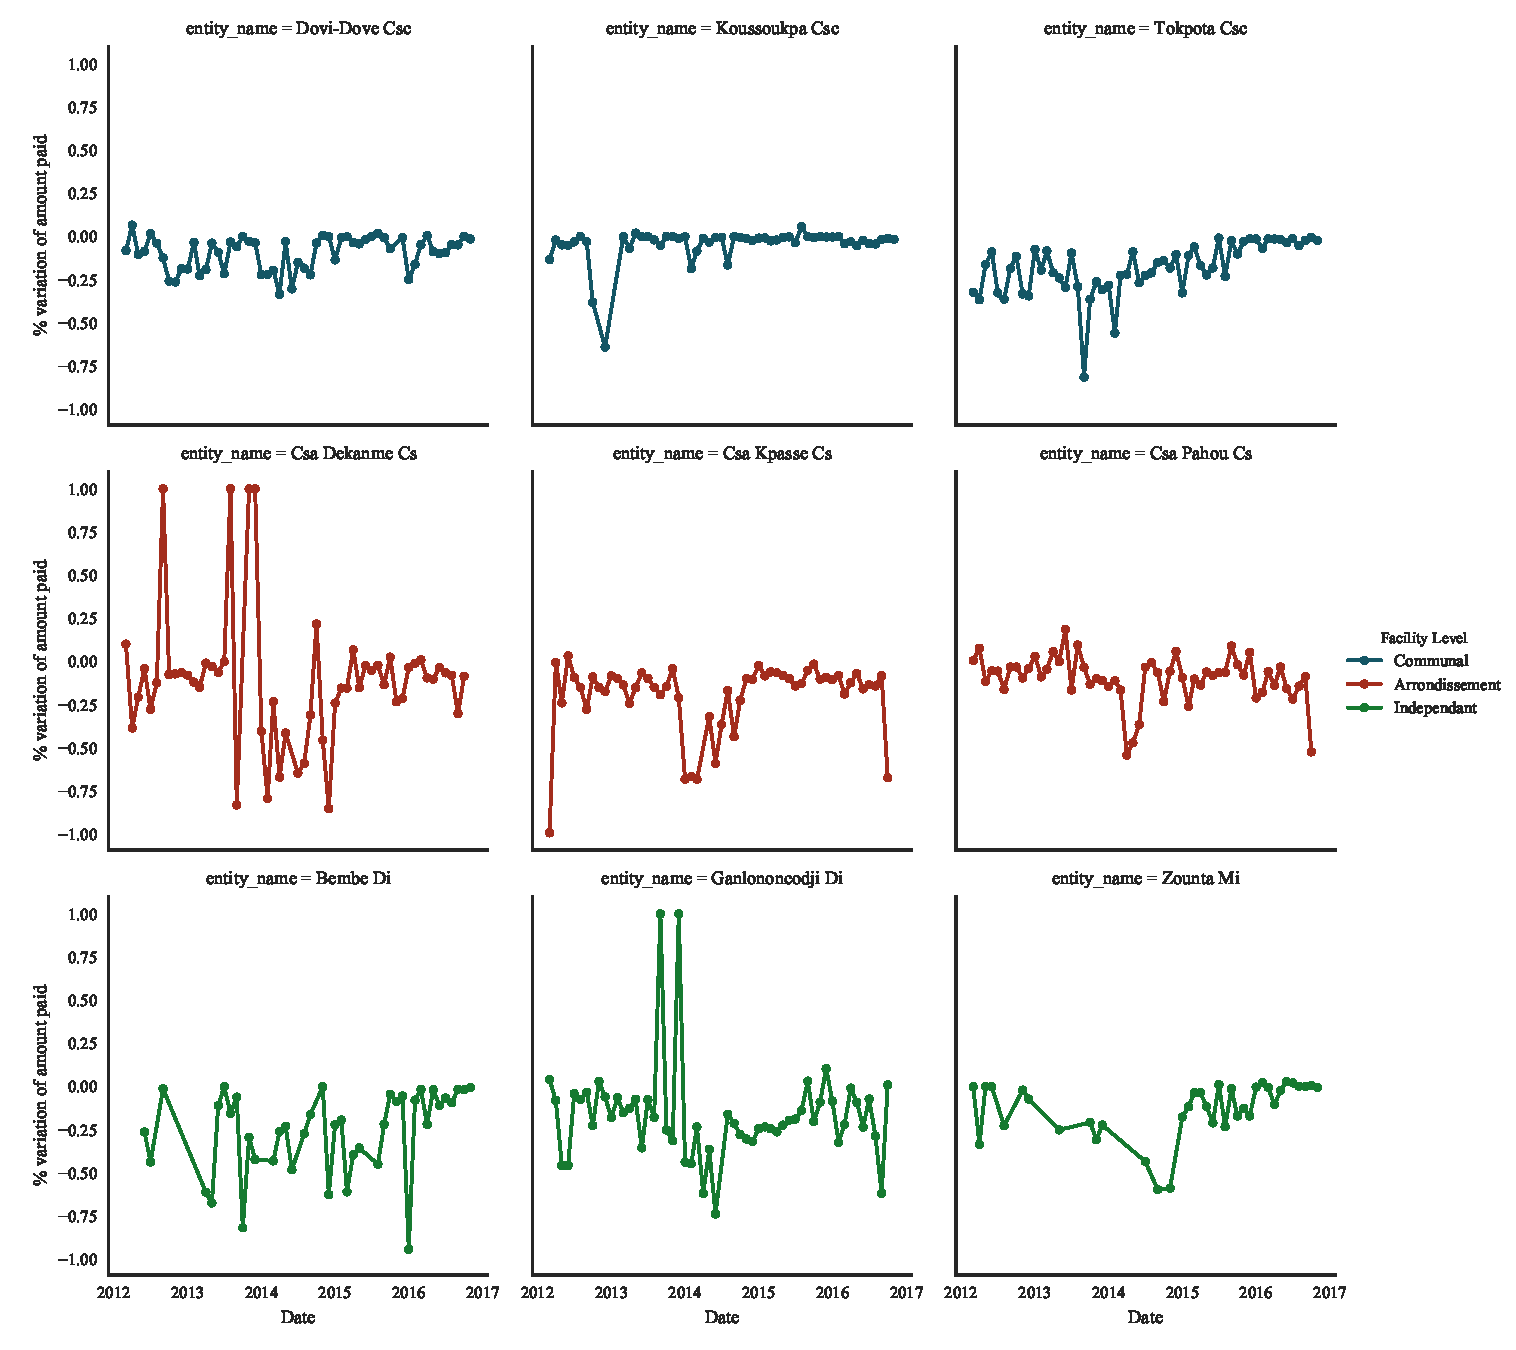
\includegraphics[width=\textwidth]{figure/facility_correction_evolution.pdf}
\caption{Evolution of payment correction percentage for a sample of indicators}
\label{fig:facility_correction_evolution}
\end{figure}
\end{center}

\subsection{Methods}
\label{sec:aim3_Methods}

\subsubsection{Theoretical Framework}
\label{sec:aim3_theoretical_framework}

Each month, each facility sends a report, composed of indicators. Each indicator $I$ has a unitary cost $C$. Thus, on month $t$, facility $f$ will receive a payment of the amount :
$$P_{t,f} = \sum_i I_{i,t,f} C_{i,t,f}$$

When taking into consideration a monthly report from a facility, we want to measure the marginal and joint probabilities of two events $Q$ and $D$, where :
\begin{enumerate}
	\item $Q = 1$ if the quality of care in the facility appears in accordance with the quality in other facilities.
	\item $D = 1$ if the data appears of sufficient quality to base payment of the facility on it.
\end{enumerate}

We are thus most interested in three distinct joint events :
\begin{itemize}
	\item $D = 0$ the data appears to be of insufficient quality to draw conclusions
	\item $D = 1 \cap Q = 0$ the data appears sufficient but quality of service seems poor
	\item $D = 1 \cap Q = 1$ the data appears sufficient and quality of service seems good
\end{itemize}


The definition of $D$ results from a budgetary arbitrage. A report is considered of insufficient quality if the expected monetary value of the payment made to facility based on this report is too severely affected by data quality. We are then interested in the difference between the payment based on reported data ($\bar{P}$) and the expected payment based on all validated information available ($P^{*}$).


I will approach this problem in two steps. I will first test multiple approaches for process monitoring, to detect and spot unlikely data patterns. I will then define a approach to classify detected abnormalities as either $D = 0$ or $D = 1 \cap Q = 0$.

\subsubsection{Data Screening}
\label{sec:data_screening}

Methods for continuous data inspection and screening come from the industrial statistics domain and are increasingly applied for healthcare monitoring \citep{woodall_use_2006,woodall_current_2014}. Spiegelhalter et al. provided et nice overview of how these tools can be used for health systems, for three main functions of interest : rating, screening and surveillance \citep{spiegelhalter_statistical_2012}. These methods are based on the standardization of data distributions, and the analysis of observed data to detect values diverging from their expected distributions. This second stage, geared toward hypothesis testing, can be made using visual tools based on adaptation of classical charts like Shewart charts, \gls{cusum} control charts or \gls{ewma} charts. I will compare and combine three approaches to this data screening question.

\paragraph{Syndromic Surveillance} A first approach is to define the expected distribution of a given series based on its past values. This approach is widely used in syndromic surveillance, and builds on a model-based \gls{cusum} approach, where the expected count of cases for a given period is modeled based on historical data, and the \gls{cusum} is updated at each period using the forecasting errors \citep{fricker_comparing_2008}. Fricker writes a general version of model-based \gls{cusum} as monitoring $S(t)$ where :
$$ S(t) = \max(0 , S(t-1) + x(t) - k)$$

where $x(t) = \frac{Y(t) - \hat{Y}(t)}{\sigma_\epsilon}$ is a standardized prediction error for $Y(t)$ on $\sigma_\epsilon$ the variation of the model error, and $k$ is a tuning parameter that will have to be optimized to obtain detection the desired characteristics for our model, including the expected monetary cost of error.

A reference implementation of this approach was developed by Farrington et al. \citep{farrington_statistical_1996} and updated by Noufaily et al. \citep{noufaily_improved_2013}, and is implemented in $R$ \citep{salmon_advances_2016}. I will implement this approach to test its ability to detect and differentiate between data quality issues and regime changes for certain indicators series. I may also use the Z-Score aggregation approach described in \citep{bardsley_using_2009} to aggregate multiple indicators result for a given facility month.

\paragraph{Hierarchical Modeling} A second approach defines expected values from a facility based on a hierarchical model including all facilities. Using Bayesian hypothesis testing strategies based on multiple sampling from the posterior distribution of facility level random effects from this hierarchical model, this approach allows me to spot unlikely numbers for a given facility as well as facility level unusual performances for a given indicator \citep{ohlssen_hierarchical_2007}.
For time $t^{*}$, $\tilde{I}_{i,t^{*},f}$ will be simulated by first simulating parameters $\alpha_f$ and $\beta_i$ and second drawing from the corresponding Poisson distribution using the different parameters.

\paragraph{Profile Monitoring} Finally, we want to be able to detect pattern variations in reports. Indeed, the methods we described until now are targeted at monitoring univariate series for which desirable variations are clearly identified. In \textit{in control} situations, the number of cases of monitored diseases are expected to stay low, and mortality rates are supposed to stay low. In the monitoring of \gls{rbf} data, meanwhile, there is no clear denominator to construct rates, and there is little sense of what an \textit{in control} situation should look like for individual indicators. Profile  monitoring is an increasingly popular research area \citep{woodall_current_2014}, and has many trends and applications, but I couldn't find any application in the healthcare sector. Its main idea is to monitor how indicators in the monitored process are related by a functional relationship, instead of monitoring individual indicators. This relationship can be specified in parametric \citep{mahmoud_simple_2011} or non parametric ways\citep{chicken_nonparametric_2011}, and I will explore the options offered by the latter approach for the type of data we have.

\subsubsection{Threshold Definition}

For each of these approaches, I will need to define thresholds to define unlikely data. This threshold will be a combination of analysis of the deviation of the observed indicators from the expected distributions, and will also incorporate an element of financial risk for. We noted the constraints of the \gls{rbf}, which should aim at spending their budget efficiently, but ensure facilities have sufficient budget to operate their basic activities. I thus define the threshold of data credibility from a financial perspective as :

\begin{itemize}
\item For the upper limit, we want to identify the risk that the cost of bad data for the system exceeds a certain threshold. This can be defined as
$$ \bar{P} - P^{*} > \eta_1 \Rightarrow D = 0$$
with $\eta_1 > 0 $.

\item For the lower limit, we consider the risk of underfunding the facilities, if the payment claimed is significantly smaller than the expected payment. This can be defined as
$$  \frac{\bar{P}}{P^{*}} > \eta_2 \Rightarrow D = 0$$
with $0 < \eta_2 < 1 $.
\end{itemize}

For any given pair of thresholds ($\eta_1 , \eta_2$), for each report computed in month $t$ for facility $f$, I am thus interested in evaluating :
	$$p(D=0) = p(\bar{P} - P^{*} > \eta_1 \cup \frac{P^{*}}{\bar{P}} > \eta_2 ) $$
	$$p(D=0) = 1 - p(\bar{P} - P^{*} < \eta	_1 \cap \frac{P^{*}}{\bar{P}} < \eta_2 )$$

For any given month $t^{*}$ in the data, using validated data from previous periods $t < t^{*}$, I will sequentially evaluate each approach in this section. I will be able to evaluate the ability of each approach to identify low quality data, or data that is too different from expected its values.

\bigskip

Using standard diagnostic evaluation methods,  I will test and evaluate the ability of each approach to properly identify aberrant data. I will also test the benefit of combining these different approaches to improve the diagnostic performances. Once this will be done, I will try to give a better understanding of whether the spotted abnormalities are due to a data quality issue, or to problems in health services provision.

\subsubsection{Risk Classification}

As described in section \ref{sec:aim3_theoretical_framework}, I am intersted in differentiating as much as possible between three situations :
\begin{itemize}
	\item $D = 0$ the data appears to be of insufficient quality to draw conclusions
	\item $D = 1 \cap Q = 0$ the data appears sufficient but quality of service seems poor
	\item $D = 1 \cap Q = 1$ the data appears sufficient and quality of service seems good
\end{itemize}

The first step of the work, by screening out situations that appear to be \textit{in control}, will allow me to rule out situations that appear to be $D = 1 \cap Q = 1$. Meanwhile, I still want to differentiate between $D = 0$ and $D = 1 \cap Q = 0$ for situations that have raised an alarm during data screening. For any indicator or report spotted as behaving in an unexpected way, I will want to understand if the problem detected can be linked to data quality issues or to a modification of the conditions of care in the facility.

I will try to solve this question by handling it as a classification problem. Using the confirmation data, I will be able to classify data as $D = 1$ or $D = 0$. Using a combination of the outputs of each data screening method  as features I will implement and test simple supervised classification methods, to differentiate between $D = 0$ and $D = 1$ in abnormal data. This second layer of classification will thus allow me to differentiate between the $D = 0$ and $D = 1 \cap Q = 0$  situations of abnormal observed data.

\subsubsection{Validation and Supervision Planning optimization}

Performing algorithmic verification comes with a risk of creating reinforcing errors. Since we fit the expected distribution of $I_i$ using only the data that was previously validated on the field, the periodic creation of such validation data points for every facilities is essential to ensure these expected distributions are still in line with reality. Meanwhile, in facilities that demonstrate good measured data quality, data will be verified less frequently than previously. This holds potential risks for our approach to be able to detect variations in performance. The question we know ask is thus, what is the minimum of validated data that has to be available in a facility to allow algorithmic validation to perform well ?

The question at stake here is to find a best performing arbitrage between data verification costs and benefits of verification. To identify a best performing data validation strategy, we will compare four strategies :

\begin{enumerate}
	\item \textbf{Reactive validation only :} On site data validation is only performed in facilities were data quality issues have been suspected algorithmically.
	\item \textbf{Reactive and yearly validation :} On site data validation is performed in facilities in which data issues have been suspected, but every facility has to be visited at least once per year.
	\item \textbf{Reactive and bi-annual validation :} Same as the previous scenario, but every facility has to be visited at least once per semester.
	\item \textbf{Reactive and quarterly validation :} Same as the previous scenario, but every facility has to be visited at least once per quarter.
\end{enumerate}

The comparison will be made by simulating progressively the implementation of each strategy on the available data. We will be describing the performances of each approach in the same way we described the performance of the full model in section \ref{sec:data_screening}.

\subsection{Timeline}
\label{timeline:aim3}

The data for this aim is already available and has been partially cleaned. I envision needing four months to implement the different data monitoring approaches, and four months for risk classification and supervision planning optimization.

\begin{figure}[t]
	\begin{ganttchart}[vgrid,hgrid,
	y unit chart=.6cm]{1}{18}
		\gantttitle{2017}{12}
		\gantttitle{2018}{6} \\
		\gantttitlelist{1,...,12}{1} \gantttitlelist{1,...,6}{1}\\

		\ganttset{bar/.append style={draw=blue!40 , fill=blue!40},
                    group/.append style={draw=blue, fill=blue}}
        \ganttbar{Data Extraction}{1}{1} \\
		\ganttbar{Data Screening}{2}{7} \\
		\ganttmilestone{Sharing Data Screening results}{7} \\
		\ganttbar{Risk Classification}{8}{9} \\
		\ganttmilestone{Risk classification results}{9} \\
		\ganttbar{Supervision Planning optimization}{10}{11} \\
		\ganttmilestone{Sharing Final Results}{11} \\
		\ganttbar{Paper Writing}{12}{14} \\
		\ganttmilestone{Paper Submission}{14}
	\end{ganttchart}
	\caption{Gantt Chart for Aim 2}
	\label{Gantt2}
\end{figure}
